\documentclass[tikz, border=15pt]{standalone}
\usetikzlibrary{arrows.meta}

\begin{document}

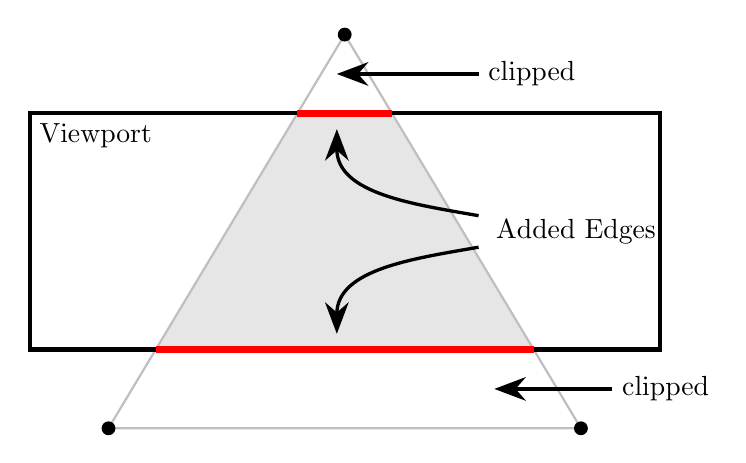
\begin{tikzpicture}[font=\sffamily]

    % Define custom colors
    \definecolor{shadedgray}{RGB}{230, 230, 230}
    
    % 1. Shaded interior (clip a filled triangle to the viewport)
    \begin{scope}
        \clip (0,1) rectangle (8,4);
        \fill[shadedgray] (4,5) -- (1,0) -- (7,0) -- cycle;
    \end{scope}

    % 2. Original triangle outline (light gray)
    \draw[lightgray, thick] (4,5) -- (1,0) -- (7,0) -- cycle;

    % 3. Viewport (thick black outline)
    \draw[line width=1.5pt] (0,1) rectangle (8,4);

    % 4. Red added edges (exact intersection coordinates)
    % Top edge: y=4. Intersections at x=3.4 and x=4.6
    \draw[red, line width=2.5pt] (3.4, 4) -- (4.6, 4);
    % Bottom edge: y=1. Intersections at x=1.6 and x=6.4
    \draw[red, line width=2.5pt] (1.6, 1) -- (6.4, 1);

    % 5. Triangle vertices (black dots)
    \fill (4,5) circle (2.5pt);
    \fill (1,0) circle (2.5pt);
    \fill (7,0) circle (2.5pt);

    % 6. Labels and Arrows
    % Viewport label
    \node[below right, font=\normalsize] at (0,4) {Viewport};

    % "clipped" top
    \node[right, font=\normalsize] (CT) at (5.7, 4.5) {clipped};
    \draw[-{Stealth[length=4mm, width=3mm]}, line width=1.2pt] (CT.west) -- (3.9, 4.5);

    % "clipped" bottom
    \node[right, font=\normalsize] (CB) at (7.4, 0.5) {clipped};
    \draw[-{Stealth[length=4mm, width=3mm]}, line width=1.2pt] (CB.west) -- (5.9, 0.5);

    % "Added Edges"
    \node[right, font=\normalsize] (AE) at (5.8, 2.5) {Added Edges};
    % Curved arrows pointing to the red lines
    \draw[-{Stealth[length=4mm, width=3mm]}, line width=1.2pt] (5.7, 2.7) to[out=170, in=270] (3.9, 3.8);
    \draw[-{Stealth[length=4mm, width=3mm]}, line width=1.2pt] (5.7, 2.3) to[out=190, in=90] (3.9, 1.2);

\end{tikzpicture}

\end{document}